\documentclass[12pt,a4paper]{article}

% Packages Ecriture
\usepackage[T1]{fontenc}
\usepackage[utf8]{inputenc}
\usepackage{fourier}
\usepackage[scaled=0.875]{helvet} 
\renewcommand{\ttdefault}{lmtt} 
\usepackage{eurosym}
\usepackage[french]{babel}
\usepackage[np]{numprint}

% Packages Mise en page
\usepackage{geometry} % Permet la mise en page
\geometry{lmargin=1cm,rmargin=1cm,tmargin=1cm,bmargin=1cm} % Choix format et  des marges
\usepackage{fancyhdr}
\usepackage{framed} % Création d'environnements
\usepackage[framed,thmmarks]{ntheorem} % Gestions des environnements theorem
\usepackage{lastpage}

\usepackage{amsmath,amssymb,makeidx}
\usepackage{enumerate}
\usepackage[normalem]{ulem}
\usepackage{fancybox,graphicx}
\usepackage{tabularx}
\usepackage{ulem}
\usepackage{dcolumn}
\usepackage{textcomp}
\usepackage{diagbox}
\usepackage{tabularx}
\usepackage{lscape}
\usepackage{pstricks,pst-plot,pst-text,pst-tree,pstricks-add,pst-grad,pst-coil,pst-blur}
\usepackage[pstricks]{bclogo} % Logo
%\setlength\paperheight{297mm}
%\setlength\paperwidth{210mm}
%\setlength{\textbfheight}{25cm}

\usepackage{multicol}

\usepackage{hyperref}

\usepackage{pgf,tikz,tkz-tab}
\usepackage{mathrsfs}
\usepackage{pifont}
\usetikzlibrary{arrows}

\usepackage{xcolor}
\usepackage{multicol}
\usepackage{multirow}


%%%%%%%%%%%%%%%%%%%%%%%%%%%%%%%%%%%%%%%%%%%%%%%%%%%%%%%%%%%%%%%%%%%%%%%%%%%%%%%%%%%%%%%%%%%%%%%%
%%%%%%%%%%%%%%%%%%%%%%%%%%%%%%%%%%%%%%%%%%%%%%%%%%%%%%%%%%%%%%%%%%%%%%%%%%%%%%%%%%%%%%%%%%%%%%%%

\DecimalMathComma	% Définit la virgule comme séparateur entre la partie entière et la partie décimale


\def\Oij{$\left(\textbfrm{O},~\vec{\imath},~\vec{\jmath}\right)$}
\def\Oijk{$\left(\textbfrm{O},~\vec{\imath},~\vec{\jmath},~\vec{k}\right)$}
\def\Ouv{$\left(\textbfrm{O},~\vec{u},~\vec{v}\right)$}

\newcommand{\vect}[1]{\mathchoice%
{\overrightarrow{\displaystyle\mathstrut#1\,\,}}%
{\overrightarrow{\textbfstyle\mathstrut#1\,\,}}%
{\overrightarrow{\scriptstyle\mathstrut#1\,\,}}%
{\overrightarrow{\scriptscriptstyle\mathstrut#1\,\,}}}

\newcommand{\equi}{\Leftrightarrow}
\newcommand{\pg}{\geqslant}
\newcommand{\pp}{\leqslant}
\newcommand{\dt}{\,\mathrm{d}t}
\newcommand{\dx}{\,\mathrm{d}x}

\newcommand{\N}{\mbox{${\mathbb N}$}}
\newcommand{\Z}{\mbox{${\mathbb Z}$}}
\newcommand{\Q}{\mbox{${\mathbb Q}$}}
\newcommand{\R}{\mbox{${\mathbb R}$}}
\newcommand{\C}{\mbox{${\mathbb C}$}}

%Commande pour créer des lignes de pointillés
\newcommand{\Pointilles}[1][3]{%
\multido{}{#1}{\makebox[\linewidth]{\dotfill}\\[\parskip]
}}

\DeclareMathOperator{\e}{e} %Permet d'écrire "droit" le e de l'exponentielle

\let\oldarray=\array
\def\array{\small\oldarray} % Permet d'écrire plus petit dans le tableau

\renewcommand{\arraystretch}{1.2} % Permet de gérer la hauteur des lignes des tableaux

\parindent=0mm % Supprime l'alinéa

\setlength{\fboxsep}{2mm} % Gère l'espacement entre un cadre et son contenu

\renewcommand{\thesection}{\Roman{section}.} % Numérote les sections en chiffre romain
\renewcommand{\thesubsection}{\Alph{subsection}.}

\newcounter{nexo}
\setcounter{nexo}{0}
\newcommand{\exo}{%
\stepcounter{nexo}
{\textbf{\underline{\textsc{Exercice \arabic{nexo}}}}%
\medskip%
}
}

\newcommand{\titre}[1]{\begin{center} {\large \framebox{\textbf{#1}}} \end{center} \medskip}


\providecommand{\tightlist}{%
  \setlength{\itemsep}{0pt}\setlength{\parskip}{0pt}}
%\providecommand{\tightlist}{\setlength{\itemsep}{25pt}\setlength{\parskip}{10pt}}

\begin{document}

\setlength\parindent{0mm}

\fancyhf{\footnotesize{}}
\fancyhead[L]{\footnotesize{}}
\fancyhead[R]{\footnotesize{}}
\fancyfoot[L]{\small{\textbf{}}}
\fancyfoot[R]{\small{\textbf{}}}

%\cfoot{Page \thepage\ sur \pageref{LastPage}}

\renewcommand{\headrulewidth}{0pt}
\renewcommand{\footrulewidth}{0pt}

\renewcommand{\labelitemi}{$\bullet$}

\pagestyle{fancy}

\titre{Feuille d'exercices 1 - Alignement de points}

Cette feuille d'exercices est à traiter après avoir lu complètement le
diaporama du cours.

\exo

Dans le repère ci-dessous, on a tracé deux droites \(d\) et \(d'\).

\begin{center}
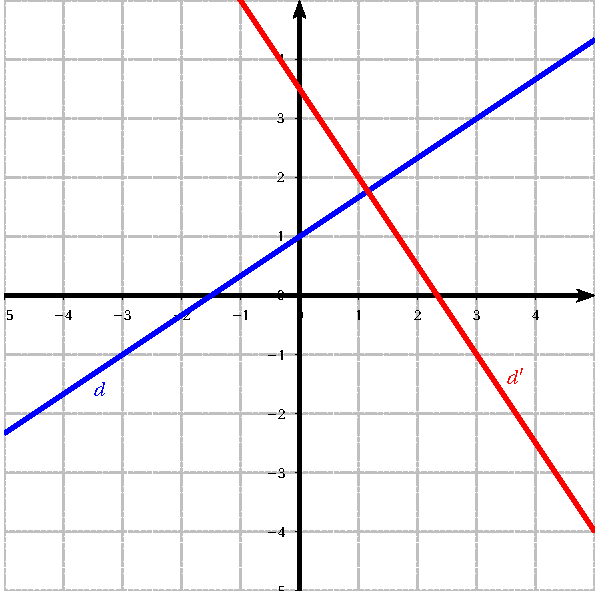
\includegraphics[scale=1]{graphique.pdf}
\end{center}

\begin{enumerate}
\def\labelenumi{\arabic{enumi}.}
\item
  \begin{enumerate}
  \def\labelenumii{(\alph{enumii})}
  \tightlist
  \item
    Déterminer par lecture graphique, un vecteur directeur de la droite
    \(d\) et un point \(A\) appartenant à la droite \(d\).

    \par

    En déduire une équation cartésienne de la droite \(d\).
  \item
    Le point \(B(93;63)\) appartient-il à la droite \(d\) ? Et le point
    \(C(-54;-35)\) ?
  \item
    Que peut-on déduire pour les points \(A\), \(B\) et \(C\) ?
  \end{enumerate}
\item
  \begin{enumerate}
  \def\labelenumii{(\alph{enumii})}
  \tightlist
  \item
    Déterminer l'équation réduite de la droite \(d'\).
  \item
    Montrer que les points \(D(-13;23)\) et \(E(29;-40)\) appartiennent
    à la droite \(d'\).
  \item
    Soit le point \(F(41;-60)\). Les droites \(D\), \(E\) et \(F\)
    sont-ils alignés ? Jusitifer.
  \end{enumerate}
\end{enumerate}

\medskip

\exo

Dans chacune des questions suivantes, déterminer si les points \(A\),
\(B\) et \(C\) sont alignés.

\begin{enumerate}
\def\labelenumi{\alph{enumi}.}
\tightlist
\item
  \(A(-6;2)\), \(B(1;1)\) et \(C(4;2)\) ;
\item
  \(A(1;4)\), \(B(-1;-6)\) et \(C(2;9)\).
\end{enumerate}

\medskip

\exo

Soient les points \(A(-1;-2)\) et \(B(1;4)\).

\begin{enumerate}
\def\labelenumi{\arabic{enumi}.}
\tightlist
\item
  Déterminer une équation cartésienne de la droite \((AB)\).
\item
  Le point \(C(-3;-9)\) est-il aligné avec les points \(A\) et \(B\) ?
  Qu'en est-il du point \(D(0;1)\).
\item
  Déterminer les réels \(y_F\) et \(x_G\) pour que les points
  \(F(3;y_F)\) et \(G(x_G;-5)\) soient alignés avec \(A\) et \(B\).
\end{enumerate}

\medskip

\newpage

\textbf{Exercice 1}

On considère la suite \((u_n)\) définie pour tout entier naturel \(n\)
par \(u_n = 2n-3\).

\begin{enumerate}
\def\labelenumi{\arabic{enumi})}
\tightlist
\item
  Calculer \(u_0\) et \(u_1\).
\item
  La suite \((u_n)\) est-elle géométrique ? Justifier
\item
  Calculer le cinquième terme de cette suite.
\end{enumerate}

\bigskip

\textbf{Exercice 2}

On considère la suite \((u_n)\) définie pour tout entier naturel \(n\)
par \(u_n = 2n-3\).

\begin{enumerate}
\def\labelenumi{\arabic{enumi}.}
\tightlist
\item
  Calculer

  \begin{enumerate}
  \def\labelenumii{\alph{enumii}.}
  \tightlist
  \item
    la valeur de \(u_0\).
  \item
    la valeur de \(u_1\).
  \end{enumerate}
\item
  La suite \((u_n)\) est-elle géométrique ? Justifier
\item
  Calculer le cinquième terme de cette suite.
\end{enumerate}

\bigskip

\textbf{Exercice 3}

Dans chacune des questions suivantes, déterminer si les points \(A\),
\(B\) et \(C\) sont alignés.

\begin{enumerate}
\def\labelenumi{\alph{enumi}.}
\tightlist
\item
  \(A(-6;2)\), \(B(1;1)\) et \(C(4;2)\) ;
\item
  \(A(1;4)\), \(B(-1;-6)\) et \(C(2;9)\).
\end{enumerate}


\end{document}